\documentclass[thesis.tex]{subfiles}
\begin{document}

\chapter{Evaluation}
\label{chap:evaluation}

Dieses Kapitel beschäftigt sich mit der Evaluation des implementierten Algorithmus. Dabei wird ausschließlich die Qualität der Bilder berücksichtigt und die Berechnungszeit ausgeklammert, da diese im Falle des Path Tracings stark von der gewählten Konfiguration und der zu rendernden Szene abhängt. Während einfache Szenen, die durch Environment Maps beleuchtet werden, in Echtzeit gerendert werden können, benötigen Szenen mit komplexen Lichtsituationen, einer hohen Anzahl an Samples und großen Pfadlängen einige Minuten zum Berechnen des Bildes. Da die Evaluation jedes denkbaren Szenarios über den Rahmen dieser Arbeit hinausgehen würde, wurde hier auf die Evaluation der Berechnungszeiten verzichtet.

Der letzte Abschnitt beschäftigt sich mit dem Vergleich zu anderen Forschungsarbeiten, die dasselbe Ziel verfolgen. Da ein direkter und ausführlicher Vergleich mit anderen Untersuchungen zu viel Raum einnehmen würde, erfolgt ein skizzenhafter Vergleich der Ergebnisse.

\section{Vergleich der Simulation mit der Kinect v2}

\begin{figure}[h!]
\centering
\begin{subfigure}{0.49\textwidth}
    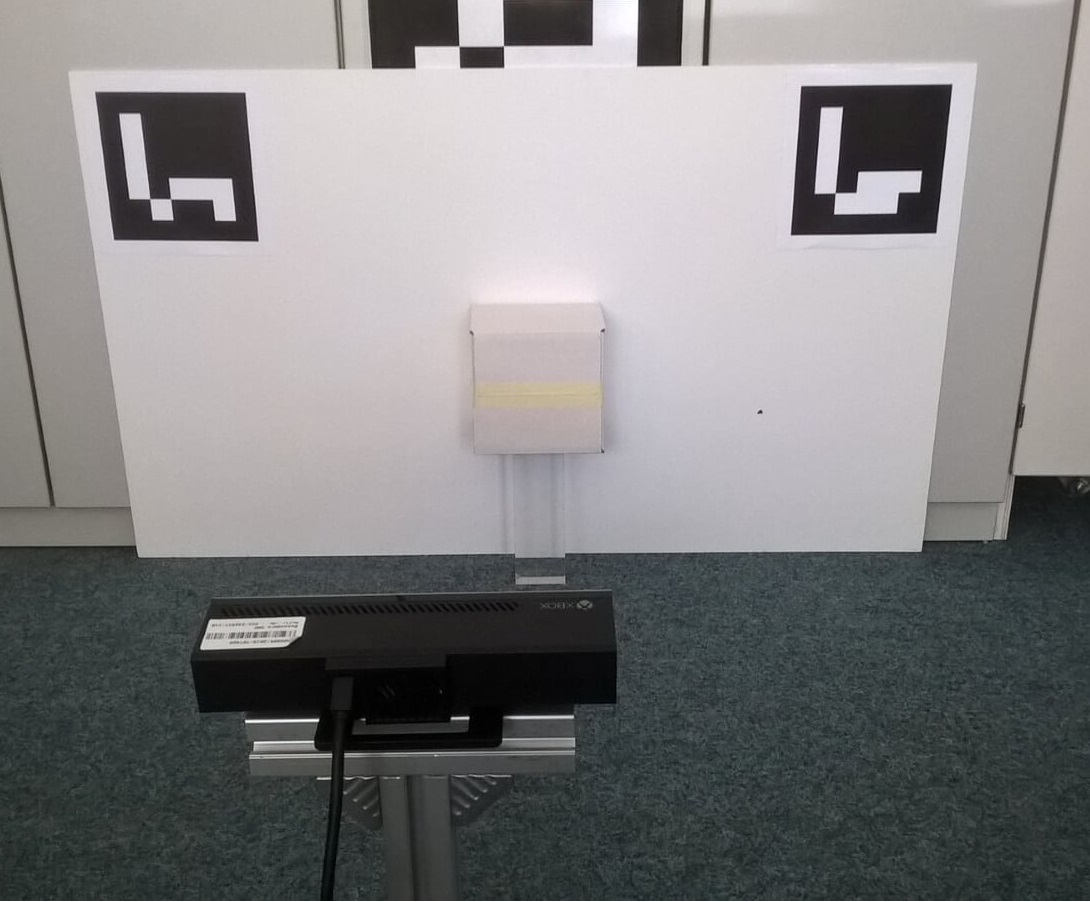
\includegraphics[width=\textwidth]{evaluation/evaluation_test_setup}
    \caption{Testaufbau mit der Kinect v2}
\end{subfigure}
\begin{subfigure}{0.49\textwidth}
    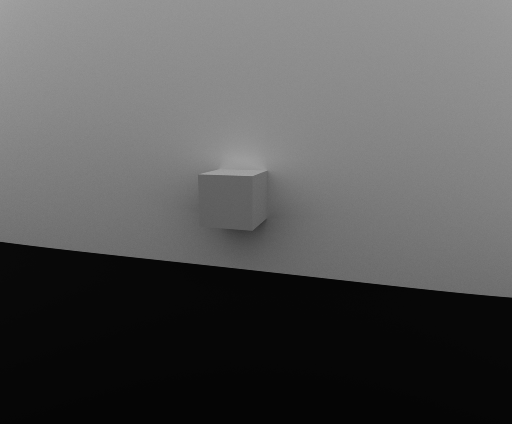
\includegraphics[width=\textwidth]{evaluation/lens_scattering_test_image}
    \caption{Testaufbau der Simulation}
\end{subfigure}
\caption{Versuchsaufbau mit der Kinect v2 und einer vereinfachten Szene innerhalb der Simulation}
\label{fig:testsetup_kinect_v2_and_simulation}
\end{figure}

In diesem Unterkapitel wird das Ergebnis der Simulation mit echten Tiefenwerten der Kinect v2 verglichen. Dazu wurde ein Testszenario aufgebaut, in dem ein quadratischer Karton vor einen stark reflektierenden Hintergrund positioniert wurde. Diese Szene wurde anschließend in einer vereinfachten Form in der Simulation nachgebildet und die Kamera wurde ähnlich positioniert (siehe \autoref{fig:testsetup_kinect_v2_and_simulation}). Zum Vergleich wurde zunächst ein Tiefenbild des Hintergrundes ohne Karton aufgenommen und anschließend eine Aufnahme mit Karton angefertigt. Anschließend wurden sowohl für die Simulation und für die Aufnahmen der Kinect v2 die Tiefenwerte miteinander verglichen und der Fehler ermittelt, der durch den Karton verursacht wurde.

\begin{figure}[h!]
\centering
\begin{subfigure}[b]{0.98\textwidth}
    \centering
    \includepdftex{scala_0_to_100}
\end{subfigure}
\vspace{5mm}
\begin{subfigure}{0.49\textwidth}
    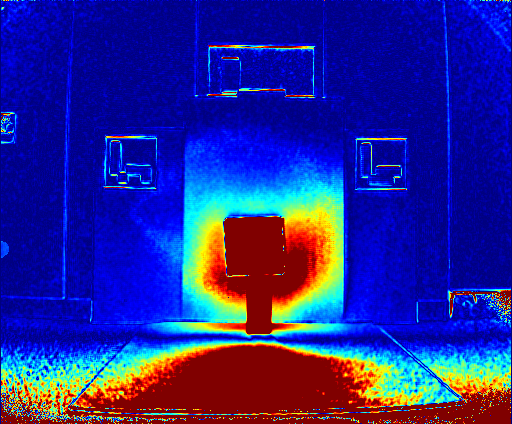
\includegraphics[width=\textwidth]{evaluation/lens_scattering_error_kinect_v2}
    \caption{Kinect v2}
\end{subfigure}
\begin{subfigure}{0.49\textwidth}
    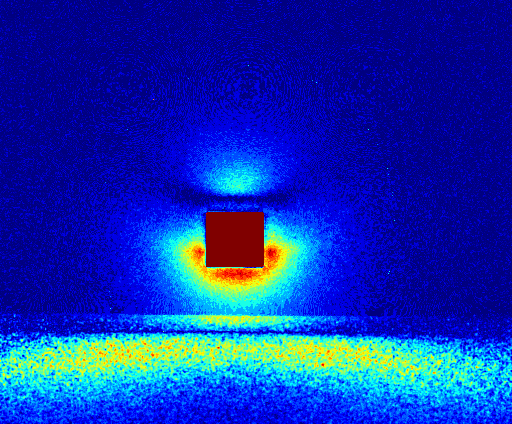
\includegraphics[width=\textwidth]{evaluation/lens_scattering_error_simulation}
    \caption{Simulation}
\end{subfigure}
\caption{Vergleich des Fehlers der Tiefenwerte der Simulation mit echten Tiefenwerten der Kinect.}
\label{fig:results_kinect_v2_and_simulation}
\end{figure}

In der \autoref{fig:results_kinect_v2_and_simulation} ist die Abweichung der Tiefenwerte nach der Positionierung des Kartons deutlich zu erkennen. Dabei ist anzumerken, dass die Rauheit und die optische Dichte der untersuchten Materialien nicht bekannt waren. Da die Analyse der Materialien im Rahmen der Arbeit nicht vorgenommen wurde, um dem vorgegebenen Rahmen der Untersuchung zu entsprechen, wurden daher plausible Werte für die Rauheit sowie die optische Dichte und den Reflexionsgrad gewählt, die allerdings nicht auf Messungen basieren, weshalb keine exakten Übereinstimmungen erwartet wurden. Das Ergebnis der Simulation zeigt, dass Abweichungen vorhanden sind, die allerdings wie erwartet in ihrer Intensität deutlich von den Ergebnissen der echten Aufnahme abweichen, da die Materialeigenschaften nicht übereinstimmen. Dennoch ist zu sehen, dass die Positionen, an denen die Abweichungen vorhanden sind, teilweise übereinstimmen, was besonders am Boden und unterhalb des Kartons zu erkennen ist. Diese Abweichungen am Boden werden überwiegend durch indirekte Beleuchtungen verursacht, während die Abweichungen in direkter Umgebung des Kartons überwiegend dem Lens Scattering zuzuschreiben sind.

\begin{figure}[h!]
\centering
\begin{subfigure}{0.49\textwidth}
    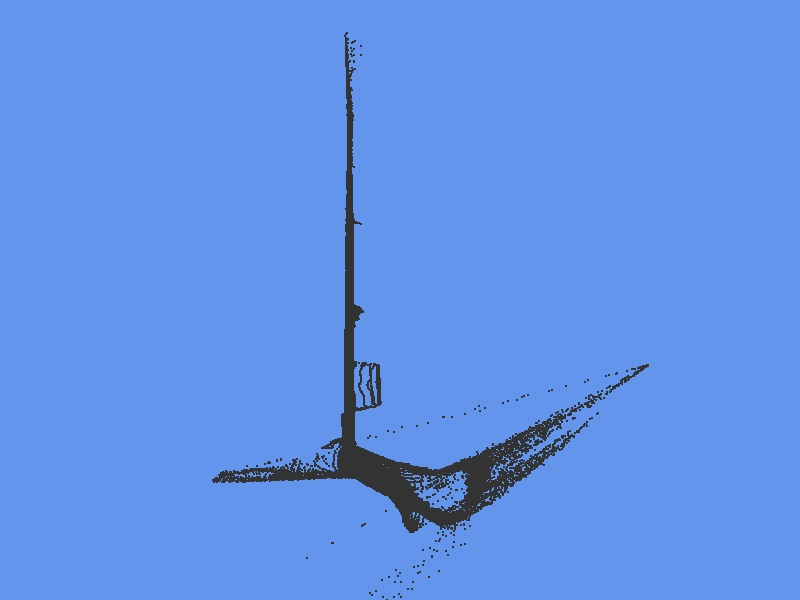
\includegraphics[width=\textwidth]{evaluation/ground_distortion}
\end{subfigure}
\caption{Aufnahme des Testaufbaus, die mit der Kinect v2 angefertigt wurde.}
\label{fig:ground_distortion}
\end{figure}

Besonders starke Abweichungen finden sich im unteren Bildbereich, die durch starke indirekte Beleuchtung verursacht wird, wodurch die Punktewolke des Bodens deutlich verfälscht wird. \autoref{fig:ground_distortion} zeigt die verfälschten Tiefenwerte des Bodens. Da die Vignettierung der Lichtquelle in der Simulation nicht nachgebildet wurde und der Boden in der Simulation daher stärtker direkt beleuchtet wird, ist diese Verzerrung schwächer ausgeprägt, was vergleichend in \autoref{fig:results_kinect_v2_and_simulation} zu sehen ist.

\section{Lens Scattering und Mixed Pixels Fehler}\label{sec:evaluation_lens_scattering}

\begin{figure}[h!]
\centering
\begin{subfigure}{0.49\textwidth}
    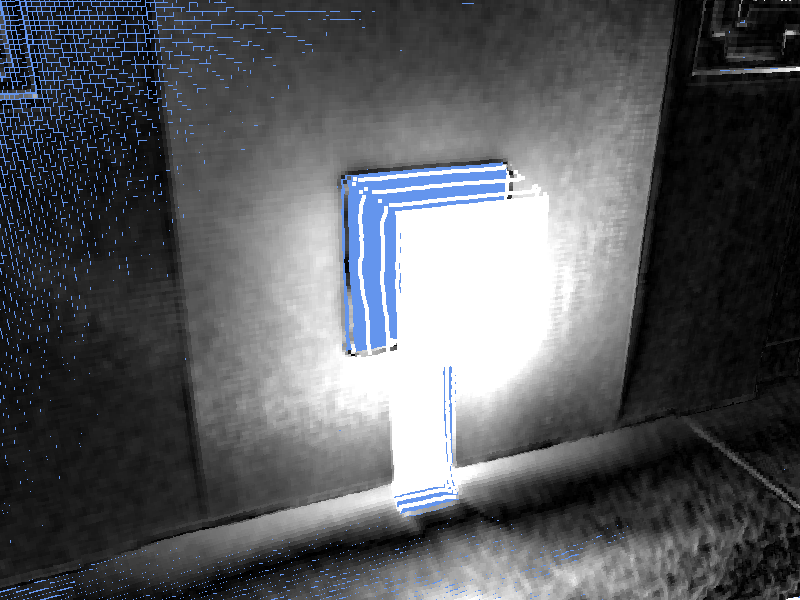
\includegraphics[width=\textwidth]{evaluation/kinect_original_2}
    \caption{Ohne Simulation von Lens Scattering}
\end{subfigure}
\caption{Fliegende Pixel, die durch Lens Scattering und Mixed Pixels verursacht wurden.}
\label{fig:flying_pixels_kinect_original}
\end{figure}

In \autoref{sec:ray_generation_simulation} wurde erläutert, dass zum Rendern eines Pixels mehrere Samples mit Strahlen in unterschiedliche Richtungen berechnet wurden. Dies führt zwar dazu, dass Mixed Pixels Fehler verursacht werden. Das reicht allerdings nicht, um Ergebnisse zu erzeugen, die mit der Aufnahme der Kinect v2 vergleichbar sind. In \autoref{fig:flying_pixels_kinect_original} wird anhand einer Aufnahme des Versuchsaufbaus gezeigt, wie die fliegenden Pixel durch Lens Scattering und Mixed Pixels verursacht werden.

\begin{figure}[h!]
\centering
\begin{subfigure}{0.49\textwidth}
    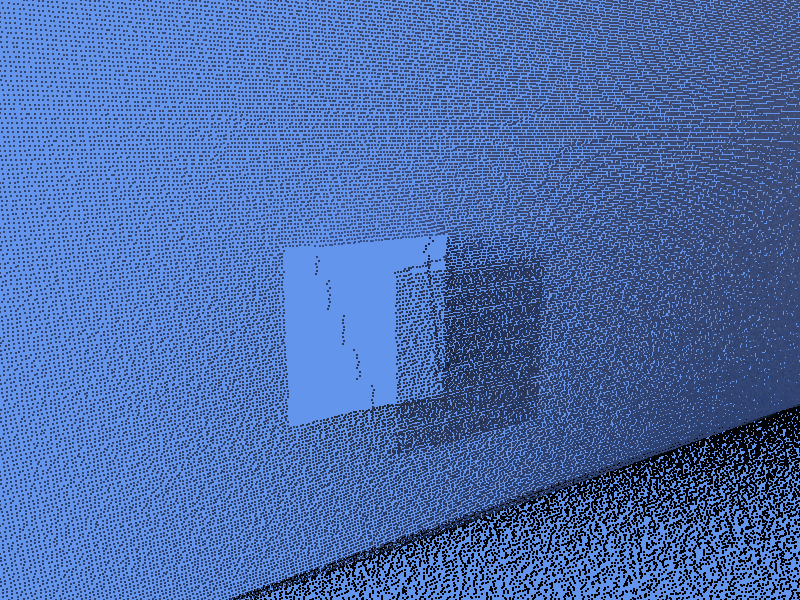
\includegraphics[width=\textwidth]{evaluation/simulation_mixed_pixels}
    \caption{Ohne Simulation von Lens Scattering}
    \label{fig:simulation_without_lens_scattering}
\end{subfigure}
\begin{subfigure}{0.49\textwidth}
    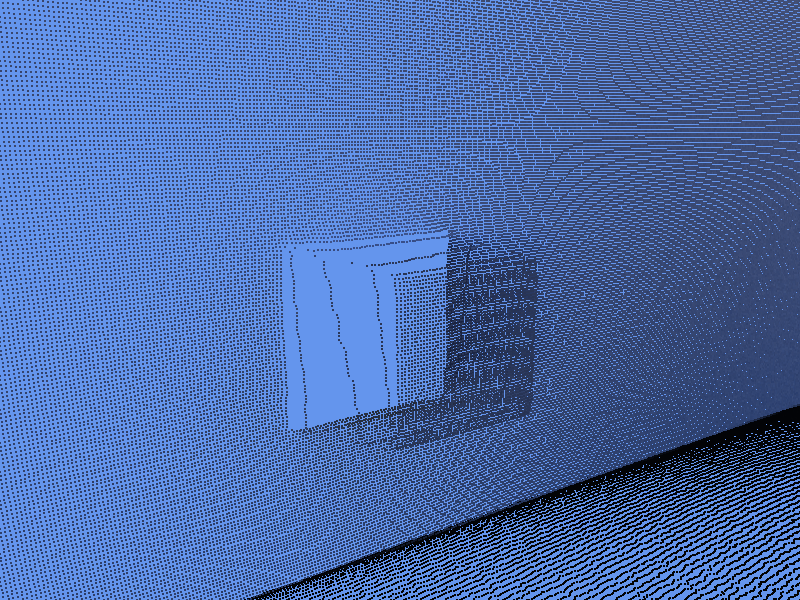
\includegraphics[width=\textwidth]{evaluation/simulation_lens_scattering}
    \caption{Mit Simulation von Lens Scattering}
    \label{fig:simulation_with_lens_scattering}
\end{subfigure}
\caption{Vergleich des Fehlers der Punktewolke der Simulation mit der gemessenen Punktewolke der Kinect.}
\label{fig:simulation_mixed_pixels_and_lens_scattering}
\end{figure}

In \autoref{fig:simulation_without_lens_scattering} sind die fliegenden Pixel zu sehen, die ausschließlich durch Mixed Pixels verursacht werden. Das Ergebnis weicht wie erwartet deutlich von dem der Aufnahme der Kinect v2 ab. Durch Berücksichtigung des Lens Scattering werden Ergebnisse erzielt, die mit den Aufnahmen der Kinect v2 übereinstimmen.

\begin{figure}[h!]
\centering
\begin{subfigure}{0.49\textwidth}
\begin{tikzpicture}
\begin{axis}[
    width=1.2\textwidth, 
    height=\axisdefaultheight,
    xmin=-600, xmax=600,
    ymin=900, ymax=1200,
    xtick={-1000},
    ytick={0},
    legend pos=north west,
    ymajorgrids=true,
    grid style=dashed,
]

\addplot+[ 
    color=red,
    mark=*,
    only marks,
    mark size=1.0pt
    ]
    table {../graphs/simulation_comparison_kinect_depth.dat};

\addplot+[ 
    color=blue,
    mark=*,
    only marks,
    mark size=1.0pt
    ]
    table [ref] {../graphs/simulation_comparison_kinect_ref.dat};
\end{axis}
\end{tikzpicture}
\caption{Echte Tiefenwerte der Kinect v2}
\end{subfigure}
\begin{subfigure}{0.49\textwidth}
\begin{tikzpicture}
\begin{axis}[
    width=1.2\textwidth, 
    height=\axisdefaultheight,
    xmin=-600, xmax=600,
    ymin=900, ymax=1200,
    xtick={-1000},
    ytick={0},
    legend pos=north west,
    ymajorgrids=true,
    grid style=dashed,
]

\addplot+[ 
    color=red,
    mark=*,
    only marks,
    mark size=1.0pt
    ]
    table {../graphs/simulation_comparison_depth.dat};

\addplot+[ 
    color=blue,
    mark=*,
    only marks,
    mark size=1.0pt
    ]
    table [ref] {../graphs/simulation_comparison_ref.dat};
\end{axis}
\end{tikzpicture}
\caption{Simulierte Tiefenwerte}
\end{subfigure}
\caption{Vergleich der gemessenen Tiefenwerte des Testaufbaus mit der Simulation.}
\label{fig:simulation_depth_compare}
\end{figure}

Neben den fliegenden Pixel verursacht das Lens Scattering außerdem, dass Tiefenwerte im Hintergrund durch stark reflektierende Objekte im Vordergrund verfälscht werden und umgekehrt. In \autoref{fig:simulation_depth_compare} werden die Tiefenwerte der Simulation mit den Aufnahmen der Kinect v2 verglichen. Die Betrachtung der Tiefenwerte der Simulation zeigt eine hohe Übereinstimmung mit den Tiefenwerten der Kinect v2. Für die Simulation wurde dafür die LED horizontal um 2,5 cm versetzt positioniert, wodurch die verfälschten Tiefenwerte im Hintergrund rechts neben der Box verursacht wurden. Zusätzlich dazu erzeugt die Simulation des Lens Scattering fliegende Pixel, die eine hohe Übereinstimmung mit den gemessenen Daten zeigen. Außerdem werden sowohl in der Simulation, als auch in den gemessenen Daten die Kanten des Kartons abgerundet und die Tiefenwerte im Hintergrund verfälscht.

\section{Multiple Path Reflexionen}

\begin{figure}[h!]
\centering
\begin{subfigure}[b]{0.98\textwidth}
    \centering
    \includepdftex{scala_0_to_100}
\end{subfigure}
\vspace{5mm}
\begin{subfigure}{0.49\textwidth}
\begin{tikzpicture}
\begin{axis}[
    width=1.2\textwidth, 
    height=\axisdefaultheight,
    xmin=-900, xmax=900,
    ymin=800, ymax=2100,
    xtick={-1000},
    ytick={0},
    legend pos=north west,
    ymajorgrids=true,
    grid style=dashed,
]

\addplot+[ 
    color=red,
    mark=none
    ]
    table {../graphs/multi_path_error_simulation_depth.dat};

\addplot+[ 
    color=blue,
    mark=none
    ]
    table [ref] {../graphs/multi_path_error_simulation_ref.dat};
\end{axis}
\end{tikzpicture}
\caption{Horizontaler Schnitt der Tiefenwerte}
\end{subfigure}
\begin{subfigure}{0.49\textwidth}
    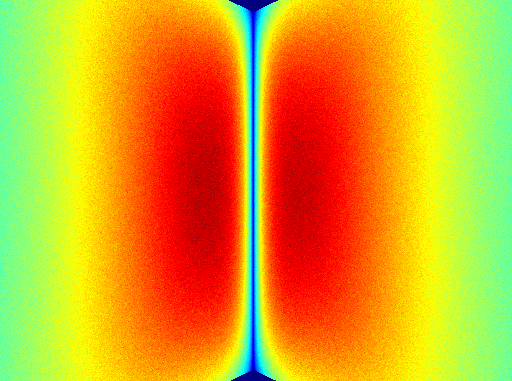
\includegraphics[width=\textwidth]{evaluation/multiple_path_error_simulation}
    \caption{Verteilung der Abweichung}
\label{fig:multiple_path_error_simulation_depth}
\end{subfigure}
    \caption{Darstellung der simulierten Tiefenwerte mit Multiple Path Fehler bei einer Pfadlänge von 16.}
    \label{fig:multiple_path_error_simulation_depth_jetmap}
\end{figure}

In \autoref{sec:multipath_problem} wurde der Fehler in Bezug auf Interreflexionen und indirekter Beleuchtung analysiert und mit den Tiefenwerten einer Punktewolke verglichen. Da es in dieser Arbeit nicht möglich war, Punktewolken in der Simulation zu rendern, wurden zum Vergleich zwei orthogonal zueinander ausgerichtete Wände vor der simulierten Kamera positioniert. \autoref{fig:multiple_path_error_simulation_depth} zeigt das Ergebnis der Simulation mit einer Pfadlänge von 16 während für die Oberfläche eine Rauheit von $\sigma = 0.5$ und eine optische Dichte von $1.52$ angesetzt wurde. In \autoref{fig:multiple_path_error_simulation_depth_jetmap} ist zu erkennen, dass die Tiefenwerte der Simulation größer sind, als die der Referenzwerte. Dieses Verhalten entspricht der Analyse, so wie es in \autoref{sec:multipath_problem} beobachtet wurde. Allerdings weicht das Ergebnis am Berührungspunkt der beiden Flächen, welcher sich im Zentrum des Bildes befindet, von den Erwartungen ab. Dies ist darauf zurückzuführen, dass Optix Schnittpunkte ignoriert, die sich zu nah am Ursprung des Strahls befinden. Dadurch werden Schnittpunkte direkt an der Kante ignoriert, was dazu führt, dass die Tiefenwerte der Simulation von denen der analysierten Kameras abweichen. Dabei handelt es sich allerdings um einen einstellbaren Parameter, welcher der Größe der Szene angepasst werden kann. Durch das Wählen eines kleineren Epsilons, das die Mindestentfernung zwischen zwei Schnittpunkten angibt, wird dieser Fehler behoben. Dies führt allerdings zu Artefakten, falls die Distanzen größer werden.

In den folgenden Abschnitten werden der Einfluss der maximalen Pfadlänge und der Rauheit der Oberfläche auf das Ergebnis im Detail untersucht.

\subsection{Fehler in Abhängigkeit zur Pfadlänge}\label{sec:eval_error_pathlength}

\begin{figure}[h!]
\centering
\begin{subfigure}{0.49\textwidth}
\begin{tikzpicture}
\begin{axis}[
    width=1.2\textwidth, 
    height=\axisdefaultheight,
    xmin=-900, xmax=900,
    ymin=800, ymax=2100,
    xtick={-1000},
    ytick={0},
    legend pos=north west,
    ymajorgrids=true,
    grid style=dashed,
]

\addplot+[ 
    color=red,
    mark=none
    ]
    table {../graphs/multi_path_length_1_depth.dat};

\addplot+[ 
    color=blue,
    mark=none
    ]
    table [ref] {../graphs/multi_path_length_1_ref.dat};
\end{axis}
\end{tikzpicture}
\caption{Maximale Pfadlänge von 2}
\end{subfigure}
\begin{subfigure}{0.49\textwidth}
\begin{tikzpicture}
\begin{axis}[
    width=1.2\textwidth, 
    height=\axisdefaultheight,
    xmin=-900, xmax=900,
    ymin=800, ymax=2100,
    xtick={-1000},
    ytick={0},
    legend pos=north west,
    ymajorgrids=true,
    grid style=dashed,
]

\addplot+[ 
    color=red,
    mark=none
    ]
    table {../graphs/multi_path_length_2_depth.dat};

\addplot+[ 
    color=blue,
    mark=none
    ]
    table [ref] {../graphs/multi_path_length_2_ref.dat};
\end{axis}
\end{tikzpicture}
\caption{Maximale Pfadlänge von 3}
\end{subfigure}
\begin{subfigure}{0.49\textwidth}
\begin{tikzpicture}
\begin{axis}[
    width=1.2\textwidth, 
    height=\axisdefaultheight,
    xmin=-900, xmax=900,
    ymin=800, ymax=2100,
    xtick={-1000},
    ytick={0},
    legend pos=north west,
    ymajorgrids=true,
    grid style=dashed,
]

\addplot+[ 
    color=red,
    mark=none
    ]
    table {../graphs/multi_path_length_3_depth.dat};

\addplot+[ 
    color=blue,
    mark=none
    ]
    table [ref] {../graphs/multi_path_length_3_ref.dat};
\end{axis}
\end{tikzpicture}
\caption{Maximale Pfadlänge von 4}
\end{subfigure}
\begin{subfigure}{0.49\textwidth}
\begin{tikzpicture}
\begin{axis}[
    width=1.2\textwidth, 
    height=\axisdefaultheight,
    xmin=-900, xmax=900,
    ymin=800, ymax=2100,
    xtick={-1000},
    ytick={0},
    legend pos=north west,
    ymajorgrids=true,
    grid style=dashed,
]

\addplot+[ 
    color=red,
    mark=none
    ]
    table {../graphs/multi_path_length_4_depth.dat};

\addplot+[ 
    color=blue,
    mark=none
    ]
    table [ref] {../graphs/multi_path_length_4_ref.dat};
\end{axis}
\end{tikzpicture}
\caption{Maximale Pfadlänge von 5}
\end{subfigure}
\caption{Vergleich der Tiefenwerte des horizontalen Schnitts von einer maximalen Pfadlänge von 2 bis 5.}
\label{fig:multiple_path_max_path_length}
\end{figure}

Bei der Simulation der indirekten Beleuchtung spielt die Wahl der maximalen Pfadlänge eine bedeutende Rolle. So erhält man bei einer Pfadlänge von 1 die Referenztiefe ohne den Einfluss indirekter Beleuchtung und ab einer Pfadlänge von 2 übt die indirekte Beleuchtung einen Einfluss auf die Tiefenwerte aus. Zur Evaluation wurden zwei orthogonal zueinander ausgerichtete Oberflächen verwendet, die ebenfalls mit einer Rauheit von $\sigma = 0.5$ und einer optischen Dichte von $1.52$ gerendert wurden. Für jede Aufnahme wurde die maximale Pfadlänge erhöht und es wurden genug Samples pro Pixel berechnet, damit das Bild vollständig berechnet wurde und sich dem korrekten Ergebnis annähert. \autoref{fig:multiple_path_max_path_length} zeigt den Vergleich der Tiefenwerte in Abhängigkeit von der maximalen Pfadlänge. Es ist zu erkennen, dass der Fehler, der durch eine indirekte Beleuchtung verursacht wurde mit der Pfadlänge zunimmt. Dabei wurde festgestellt, dass es ab einer Pfadlänge von 5 kein Unterschied zu einer Pfadlänge von 16 gibt.

\subsection{Fehler in Abhängigkeit zur Rauheit der Oberfläche}

\begin{figure}[h!]
\centering
\begin{subfigure}{0.49\textwidth}
\begin{tikzpicture}
\begin{axis}[
    width=1.2\textwidth, 
    height=\axisdefaultheight,
    xmin=-900, xmax=900,
    ymin=800, ymax=2100,
    xtick={-1000},
    ytick={0},
    legend pos=north west,
    ymajorgrids=true,
    grid style=dashed,
]

\addplot+[ 
    color=red,
    mark=none
    ]
    table {../graphs/multi_path_roughtness_1_depth.dat};

\addplot+[ 
    color=blue,
    mark=none
    ]
    table [ref] {../graphs/multi_path_roughtness_1_ref.dat};
\end{axis}
\end{tikzpicture}
\caption{$\sigma = 1.0$}
\end{subfigure}
\begin{subfigure}{0.49\textwidth}
\begin{tikzpicture}
\begin{axis}[
    width=1.2\textwidth, 
    height=\axisdefaultheight,
    xmin=-900, xmax=900,
    ymin=800, ymax=2100,
    xtick={-1000},
    ytick={0},
    legend pos=north west,
    ymajorgrids=true,
    grid style=dashed,
]

\addplot+[ 
    color=red,
    mark=none
    ]
    table {../graphs/multi_path_roughtness_4_depth.dat};

\addplot+[ 
    color=blue,
    mark=none
    ]
    table [ref] {../graphs/multi_path_roughtness_4_ref.dat};
\end{axis}
\end{tikzpicture}
\caption{$\sigma = 0.7$}
\end{subfigure}
\begin{subfigure}{0.49\textwidth}
\begin{tikzpicture}
\begin{axis}[
    width=1.2\textwidth, 
    height=\axisdefaultheight,
    xmin=-900, xmax=900,
    ymin=800, ymax=2100,
    xtick={-1000},
    ytick={0},
    legend pos=north west,
    ymajorgrids=true,
    grid style=dashed,
]

\addplot+[ 
    color=red,
    mark=none
    ]
    table {../graphs/multi_path_roughtness_7_depth.dat};

\addplot+[ 
    color=blue,
    mark=none
    ]
    table [ref] {../graphs/multi_path_roughtness_7_ref.dat};
\end{axis}
\end{tikzpicture}
\caption{$\sigma = 0.4$}
\end{subfigure}
\begin{subfigure}{0.49\textwidth}
\begin{tikzpicture}
\begin{axis}[
    width=1.2\textwidth, 
    height=\axisdefaultheight,
    xmin=-900, xmax=900,
    ymin=800, ymax=2100,
    xtick={-1000},
    ytick={0},
    legend pos=north west,
    ymajorgrids=true,
    grid style=dashed,
]

\addplot+[ 
    color=red,
    mark=none
    ]
    table {../graphs/multi_path_roughtness_10_depth.dat};

\addplot+[ 
    color=blue,
    mark=none
    ]
    table [ref] {../graphs/multi_path_roughtness_10_ref.dat};
\end{axis}
\end{tikzpicture}
\caption{$\sigma = 0.1$}
\end{subfigure}
\caption{Vergleich der Tiefenwerte des horizontalen Schnitts in Abhängigkeit zur Rauheit der Oberfläche.}
\label{fig:multiple_path_error_roughness}
\end{figure}

Zusätzlich zur Pfadlänge beeinflussen auch die Reflexionseigenschaften der Oberfläche den Fehler, der durch indirekte Reflexionen verursacht wird. Daher wurde die Simulation dahingehend näher untersucht. Dazu wurden ebenfalls wie zuvor in der Szene zwei orthogonal zueinander ausgerichtete Flächen gewählt und die Rauheit wurde variiert. Für diese Untersuchung wurde für jede Aufnahme wieder eine optische Dichte von 1.52 gewählt.

Die Ergebnisse der Untersuchung sind in \autoref{fig:multiple_path_error_roughness} zu sehen. Dabei ist zu erkennen, dass für eine Rauheit von $\sigma = 1.0$ der Fehler zunächst gering ausfällt und dieser sich für glattere Oberflächen erhöht. Dies ist damit zu erklären, dass rauere Oberflächen einen größeren Anteil der Strahlung in die Richtung der Strahlungsquelle reflektieren, was zu einer geringeren indirekten Beleuchtung für raue Oberflächen führt.

\section{Systematische Fehler}

\begin{figure}[ht!]
\centering
\begin{subfigure}{\textwidth}
\begin{tikzpicture}
\begin{axis}[
    width=\textwidth, 
    height=\axisdefaultheight,
    xlabel={Tatsächlicher Tiefenwert in mm},
    ylabel={Abweichung des Tiefenwerts in mm},
    xmin=700, xmax=3000,
    ymin=-70, ymax=70,
    xtick={700,1000,1500,2000,2500,3000},
    ytick= {-80,-60,-40,-20,0,20,40,60,80},
    legend pos=south east,
    ymajorgrids=true,
    grid style=dashed,
]

\addplot+[ 
    color=blue,
    only marks,
    mark=*,
    mark size=0.5pt
    ]
    table {../graphs/simulation_systematic_error_30mhz.dat};
\addlegendentry{30 Mhz}
\end{axis}
\end{tikzpicture}
\end{subfigure}
\begin{subfigure}{\textwidth}
\begin{tikzpicture}
\begin{axis}[
    width=\textwidth, 
    height=\axisdefaultheight,
    xlabel={Tatsächlicher Tiefenwert in mm},
    ylabel={Abweichung des Tiefenwerts in mm},
    xmin=700, xmax=3000,
    ymin=-100, ymax=100,
    xtick={700,1000,1500,2000,2500,3000},
    ytick={-100,-80,-60,-40,-20,0,20,40,60,80,100},
    legend pos=south east,
    ymajorgrids=true,
    grid style=dashed,
]

\addplot+[ 
    color=blue,
    only marks,
    mark=*,
    mark size=0.5pt
    ]
    table {../graphs/simulation_systematic_error_20mhz.dat};
\addlegendentry{20 Mhz}
\end{axis}
\end{tikzpicture}
\end{subfigure}
\caption{Systematischer Fehler bei der Simulation der Tiefenwerte mittels rechteckförmige Wellenfunktionen in Abhängigkeit zur tatsächlichen Distanz.}
\label{fig:wiggle_error_simulation_rect}
\end{figure}

Die Ermittlung des systematischen Fehlers der Simulation erfolgte analog zum Vorgehen, das in \autoref{sec:systematoc_error} beschrieben wurde. Allerdings wurden die Tiefenwerte der sinusförmiger Wellenfunktionen als Referenzwert herangezogen, da festgestellt wurde, dass die Continuous-Wave Modulation mittels sinusförmigen Wellenfunktionen keinen systematischen Fehler aufweist. Da anhand der Mehrdeutigkeitsdistanz festgestellt wurde, dass die IFM O3D03 mit einer Frequenz von 30 Mhz arbeitet und die ASUS Xtion 2 eine Frequenz von 20 Mhz verwendet, wird die Simulation mit diesen Frequenzen untersucht.

\begin{figure}[ht!]
\centering
\begin{subfigure}{\textwidth}
\begin{tikzpicture}
\begin{axis}[
    width=\textwidth, 
    height=\axisdefaultheight,
    xlabel={Tatsächlicher Tiefenwert in mm},
    ylabel={Abweichung des Tiefenwerts in mm},
    xmin=700, xmax=3000,
    ymin=-300, ymax=70,
    xtick={700,1000,1500,2000,2500,3000},
    legend pos=north east,
    ymajorgrids=true,
    grid style=dashed,
]

\addplot+[ 
    color=blue,
    only marks,
    mark=*,
    mark size=0.5pt
    ]
    table {../graphs/simulation_systematic_error_30mhz_pusled.dat};
\addlegendentry{16 ns Pulsdauer}
\end{axis}
\end{tikzpicture}
\end{subfigure}
\begin{subfigure}{\textwidth}
\begin{tikzpicture}
\begin{axis}[
    width=\textwidth, 
    height=\axisdefaultheight,
    xlabel={Tatsächlicher Tiefenwert in mm},
    ylabel={Abweichung des Tiefenwerts in mm},
    xmin=700, xmax=3000,
    ymin=-300, ymax=70,
    xtick={700,1000,1500,2000,2500,3000},
    legend pos=north east,
    ymajorgrids=true,
    grid style=dashed,
]

\addplot+[ 
    color=blue,
    only marks,
    mark=*,
    mark size=0.5pt
    ]
    table {../graphs/simulation_systematic_error_20mhz_pusled.dat};
\addlegendentry{25 ns Pulsdauer}
\end{axis}
\end{tikzpicture}
\end{subfigure}
\caption{Systematischer Fehler bei der Simulation der Tiefenwerte mittels pulsdauermodulation in Abhängigkeit zur tatsächlichen Distanz.}
\label{fig:wiggle_error_simulation_pulse}
\end{figure}

In \autoref{fig:wiggle_error_simulation_rect} ist der systematische Fehler der Simulation unter Verwendung der rechteckförmigen Amplutudenmodulation dargestellt. Dabei ist zu sehen, dass die Verwendung dieser Modulation einen sinusförmigen Fehler einführt. Die Analyse der O3D303 in \autoref{sec:systematoc_error} lässt erahnen, dass es sich bei dem Verlauf des systematischen Fehlers ebenfalls um einen Sinusverlauf handelt. Es wurde außerdem festgestellt, dass sowohl die Amplitude als auch die Wellenlänge des systematischen Fehlers von der genutzten Frequenz abhängig ist. 

Weiter wurde auch der systematische Fehler der Pulsdauermodulation untersucht. Ohne den Einfluss jeglichen Umgebungslichtes konnte ebenfalls kein Fehler festgestellt werden. Die Tiefenwerte werden bei Verwendung der Pulsdauermodulation allerdings durch Umgebungslicht beeinflusst, das durch externe Quellen wie der Sonne oder künstlicher Beleuchtung im Raum verursacht wird. \autoref{fig:wiggle_error_simulation_pulse} zeigt den Fehler der Simulation unter Einfluss von Umgebungslicht, das durch eine Environment Map verursacht wurde. Dabei sind Ähnlichkeiten zur Analyse des systematischen Fehlers der Xtion 2 zu erkennen. Daher liegt die Vermutung nahe, dass es sich bei der Xtion 2 um ein Time-of-Flight Kamerasystem handelt, das mit zwei Buckets arbeitet. Da allerdings keine Details zur internen Funktionsweise der Xtion 2 bekannt sind und eine genaue Untersuchung den Rahmen der Arbeit übersteigt, kann keine genaue Aussage darüber getroffen werden.

\section{Vergleich mit anderen Arbeiten}

In \autoref{chap:relatedwork} wurden verwandte Arbeiten erläutert, die ein ähnliches Ziel verfolgen wie die vorliegende. Dabei wurde auf die Arbeiten von Meister et al. \cite{bib:Meister2012PhotonMB}\cite{bib:Meister2013} Bezug genommen, die sich auf die Simulation der Lichtausbreitung konzentrieren. Zum einen wurde die Lichtausbreitung mittels Photon Mapping simuliert und zum anderen wurde bidirektionales Path Tracing verwendet. Dabei wurde die Linsenkrümmung nicht berücksichtigt und ausschließlich eine Continuous-Wave Modulation mit sinusförmigen Wellenfunktionen simuliert. Auch der systematische Fehler wurde nicht untersucht. Aus den Arbeiten geht ebenfalls nicht hervor, ob die Mehrdeutigkeit für größere Distanzen simuliert wurde. Im Gegensatz zu den Ergebnissen, die in \autoref{sec:eval_error_pathlength} erläutert wurden, weist die Simulation von Meister et al. \cite{bib:Meister2013} keinen Fehler am Berührungspunkt der zwei Oberflächen auf. Allerdings kommen Meister et al. zum Schluss, dass eine Pfadlänge von mindestens 8 notwendig ist, um ein Tiefenbild zu erzeugen, das sich nicht von Tiefenbildern mit Pfadlängen mit einem höheren Wert unterscheidet. Die radiale Verzeichnung und Effekte, die durch Lens Scattering verursacht werden, welche in dieser Arbeit erfolgreich simuliert werden konnten, wurden in der Simulation von Meister et al. ebenfalls nicht berücksichtigt. Es wurde außerdem angenommen, dass die LED Position mit der Position der Kamera übereinstimmt, weshalb Fehler, wie in \autoref{sec:analysis_led_position} erläutert, nicht adressiert wurden.

Keller \cite{bib:Keller2015} konzentriert sich in seiner Dissertation auf die Echtzeitsimulation eines Time-of-Flight Sensors. Dabei wurde ebenfalls auf die Simulation der Linsenkrümmung und auf Lens Scattering verzichtet. Allerdings wurden die systematischen Fehler erfolgreich simuliert. Im Gegensatz zu dieser Arbeit hat Keller den systematischen Fehler eines Kamerasystems eingemessen um es anschließend in einer Simulation angewandt. Der Fehler durch indirekte Beleuchtung und sonstige Fehler, die durch die Lichtausbreitung verursacht wurden, wurden von Keller nicht adressiert. Allerdings ist die Simulation, die Keller in seiner Dissertation beschreibt, im Gegensatz zur Simulation in dieser Arbeit echtzeitfähig. Auch wenn das progressive Path Tracing Interaktionen des Nutzers während des Renderings erlaubt, wird bedeutend mehr Rechenzeit benötigt, bis das Bild gegen das richtige Ergebnis konvergiert. Das Endresultat des Bildes wird daher nicht in Echtzeit geliefert. 

\subfilebib % Makes bibliography available when compiling as subfile
\end{document}
